\documentclass{sigchi}

% Use this command to override the default ACM copyright statement (e.g. for preprints). 
% Consult the conference website for the camera-ready copyright statement.


% Arabic page numbers for submission. 
% Remove this line to eliminate page numbers for the camera ready copy
%\pagenumbering{arabic}



\usepackage{balance}  % to better equalize the last page
\usepackage{graphics} % for EPS, load graphicx instead
\usepackage{times}    % comment if you want LaTeX's default font
\usepackage{url}      % llt: nicely formatted URLs
\usepackage{graphicx}
\usepackage{caption}
\usepackage{subcaption}
\usepackage{array}

% llt: Define a global style for URLs, rather that the default one
\makeatletter
\def\url@leostyle{%
  \@ifundefined{selectfont}{\def\UrlFont{\sf}}{\def\UrlFont{\small\bf\ttfamily}}}
\makeatother
\urlstyle{leo}


% To make various LaTeX processors do the right thing with page size.
\def\pprw{8.5in}
\def\pprh{11in}
\special{papersize=\pprw,\pprh}
\setlength{\paperwidth}{\pprw}
\setlength{\paperheight}{\pprh}
\setlength{\pdfpagewidth}{\pprw}
\setlength{\pdfpageheight}{\pprh}

% Make sure hyperref comes last of your loaded packages, 
% to give it a fighting chance of not being over-written, 
% since its job is to redefine many LaTeX commands.
%\usepackage[pdftex]{hyperref}
%\hypersetup{
%pdftitle={L@S 2014 Work-in-Progress Format},
%pdfauthor={LaTeX},
%pdfkeywords={SIGCHI, proceedings, archival format},
%bookmarksnumbered,
%pdfstartview={FitH},
%colorlinks,
%citecolor=black,
%filecolor=black,
%linkcolor=black,
%urlcolor=black,
%breaklinks=true,
%}

% create a shortcut to typeset table headings
\newcommand\tabhead[1]{\small\textbf{#1}}

\begin{document}

\title{Exploring Classification}


\maketitle

\large

\section{Support Vector Machine}

We implemented the dual form of linear SVM's with slack variables in Python. To do so, we converted the input into a quadratic program, which we used \texttt{cvxopt.solvers.qp} to solve. Recall the general form of the quadratic program for the dual form of the SVM, which is given by

\normalsize
\begin{center}\begin{tabular}{r p{0.0in} l }
maximize && $ \displaystyle \sum_{i =1}^n \alpha_i - \frac{1}{2}\sum_{i = 1}^{n}\sum_{j = 1}^n \alpha_i\alpha_jy^{(i)}y^{(j)}(x^{(i)}\cdot x^{(j)}) $
\\ && \\
subject to && $ \displaystyle 0 \leq \alpha_i \leq C$ 
\\ && \\
&&		      $ \displaystyle \sum_{i = 1}^{n} \alpha_iy^{(i)} = 0$
\end{tabular}\end{center}

\large

We will demonstrate the formulation of this program in the matrix form required for \texttt{cvxopt.solvers.qp} on a simple example. Consider the dataset with positive examples $(1, 2)$ and $(2, 2)$ and negative examples $(0, 0)$ and $(-2, 3)$.
If we order the dataset according to the order presented here, then in matrix notation, the quadratic program above is given by

\normalsize
\begin{center}\begin{tabular}{r p{0.0in} l }
minimize &&\\
&&
$ \displaystyle \frac{1}{2}\alpha^T
\begin{bmatrix}
5 & 6 & 0 & -4\\
6 & 8 & 0 & -2\\
0 & 0 & 0 & 0\\
-4 & -2 & 0 & 13\\
\end{bmatrix}
\alpha +
\begin{bmatrix}
-1\\ -1\\ -1\\ -1\\
\end{bmatrix}^T
\alpha
 $
\\ && \\
subject to &&\\
&& $
\begin{bmatrix}
1 & 0 & 0 & 0\\
-1 & 0 & 0 & 0\\
0 & 1 & 0 & 0\\
0 & -1 & 0 & 0\\
0 & 0 & 1 & 0\\
0 & 0 & -1 & 0\\
0 & 0 & 0 & 1\\
0 & 0 & 0 & -1\\
\end{bmatrix}
\alpha
\leq
\begin{bmatrix}
C\\
0\\
C\\
0\\
C\\
0\\
C\\
0\\
\end{bmatrix}
$ 
\\ && \\
&&		      $ 
\begin{bmatrix}
1& 1& -1& -1\\
\end{bmatrix}
\alpha = \begin{bmatrix}0\end{bmatrix}
$
\end{tabular}\end{center}

\large
Solving this linear program for $\alpha$, we obtain the linear separator shown in Figure 1. For this small example, we can clearly see that this separator maximizes the margin.

\begin{figure}
\centering
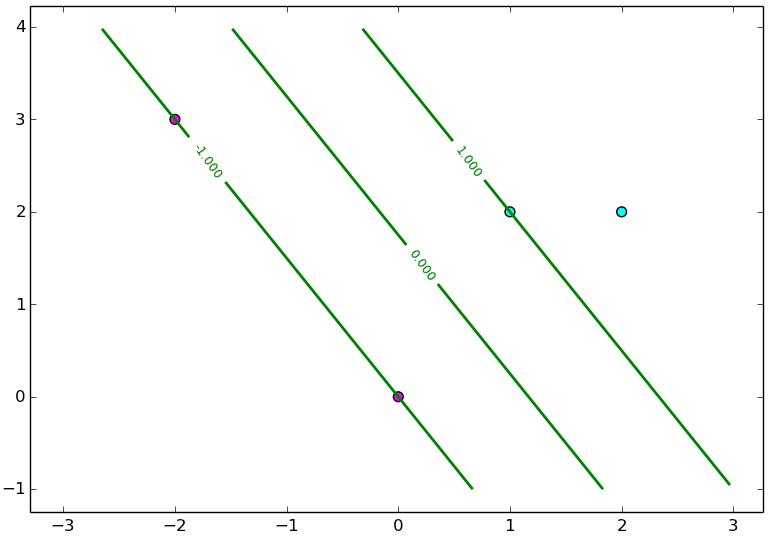
\includegraphics[width=2.25in]{plots/1-1.png}
\caption{test}
\end{figure}

Next, we test our implementation on four different data sets, each consisting of 400 points. The first three data sets, which we will refer to as \texttt{stdev1}, \texttt{stdev2}, \texttt{stdev4}, consist of points where each of the negative and positive examples are generated from a Gaussian distribution with varying standard deviations (as suggested by the name). The final data set, \texttt{nonSep}, is a data set generated as to be impossible to separate with a linear separator.

For each of these data sets we will use a value of $C = 1$, and we will show the resulting boundary on both a training and validation set. We will also report the training and validation error rates. We begin with \texttt{stdev1}.

Figures 2(a) and 2(b) show the decision boundary formed by our algorithm on the training and validation data, respectively. As we can clearly see, both the training and validation data have an error rate of 0. This is not surprising given the very large gap between positive and negative samples.

Figure 2 also shows the results of repeating the process with \texttt{stdev2} and \texttt{stdev4}. For \texttt{stdev2}, the training error rate was 9.25\% and the validation error rate was 8.25\%. For \texttt{stdev4}, the training error rate was 26.5\% and validation error rate 23.5\%.

We can clearly see from the plots that \texttt{stdev2} and \texttt{stdev4} are not linearly separable (both in training and validation data), and thus we are not surprised by the increased error rates. It is interesting to note that the training data has higher error rates than the validation data in both cases. However, since both training data and validation data were drawn from Gaussian distributions, this is not terribly unlikely and does not surprise us.

Although we will not explore this idea for the purposes of this paper, one could try to optimize the value of $C$ in order to decrease the validation error further.

\begin{figure*}[!ht]
\centering
\begin{tabular}{c c c}
\begin{subfigure}[b]{2.25in}
	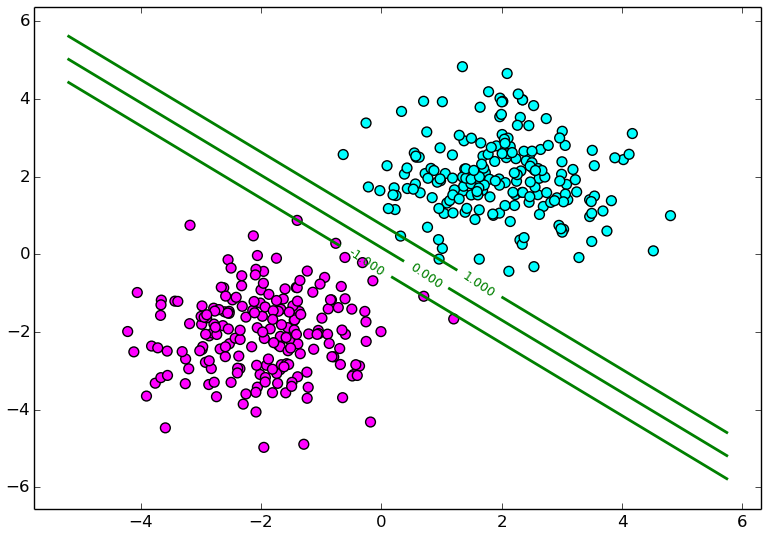
\includegraphics[width=2.25in]{plots/1-2/stdev1train.png}
	\caption{\texttt{stdev1} Training Data}
\end{subfigure} &

\begin{subfigure}[b]{2.25in}
	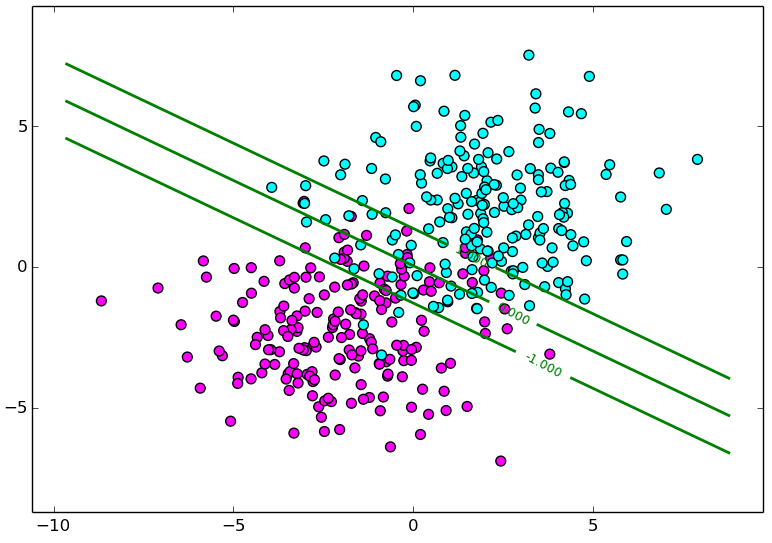
\includegraphics[width=2.25in]{plots/1-2/stdev2train.png}
	\caption{\texttt{stdev2} Training Data}
\end{subfigure} &

\begin{subfigure}[b]{2.25in}
	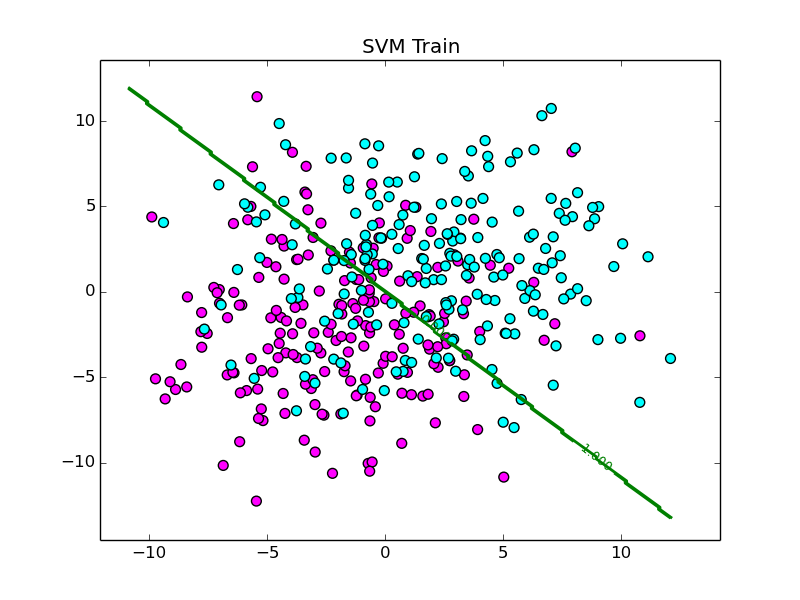
\includegraphics[width=2.25in]{plots/1-2/stdev4train.png}
	\caption{\texttt{stdev4} Training Data}
\end{subfigure} \\

\begin{subfigure}[b]{2.25in}
	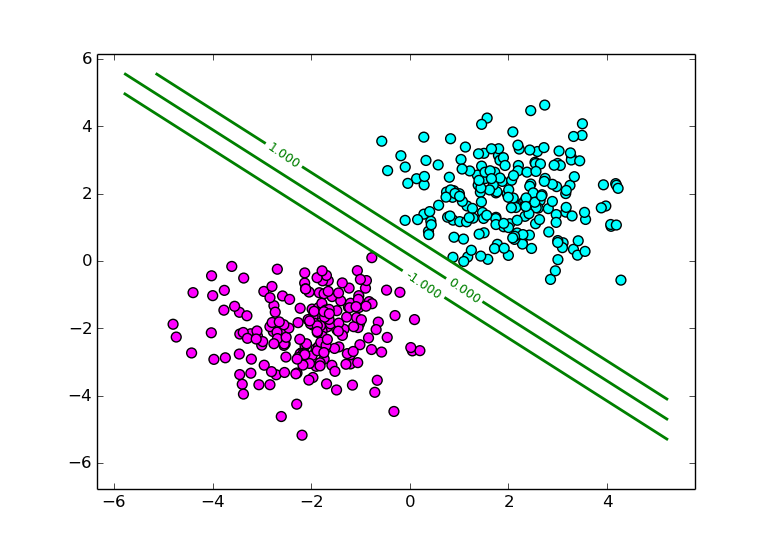
\includegraphics[width=2.25in]{plots/1-2/stdev1valid.png}
	\caption{\texttt{stdev1} Validation Data}
\end{subfigure} &

\begin{subfigure}[b]{2.25in}
	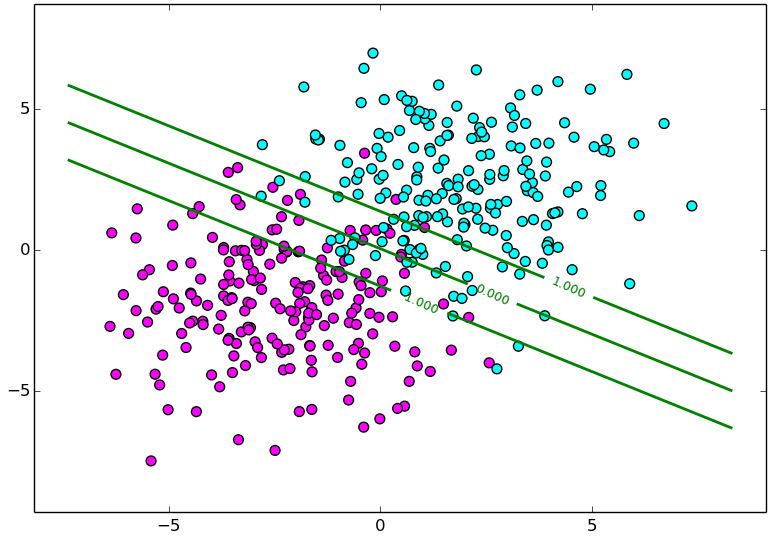
\includegraphics[width=2.25in]{plots/1-2/stdev2valid.png}
	\caption{\texttt{stdev2} Validation Data}
\end{subfigure} &

\begin{subfigure}[b]{2.25in}
	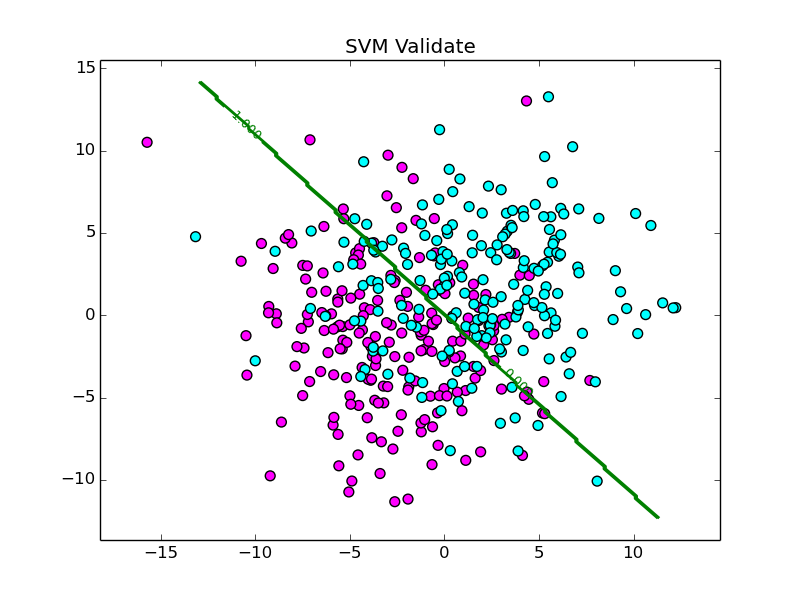
\includegraphics[width=2.25in]{plots/1-2/stdev4valid.png}
	\caption{\texttt{stdev4} Validation Data}
\end{subfigure} \\
\end{tabular}
\caption{test}
\end{figure*}

Next, we focus on \texttt{nonSep}. The resulting decision boundaries are shown in Figure 3. Clearly, this data is ill-fitted for classification via a linear separator.

\begin{figure}
\centering

\begin{subfigure}[b]{2.25in}
	\includegraphics[width = 2.25in]{plots/1-2/nonSep2train.png}
	\caption{\texttt{nonSep} Training Data}
\end{subfigure}

\begin{subfigure}[b]{2.25in}
	\includegraphics[width = 2.25in]{plots/1-2/nonSep2valid.png}
	\caption{\texttt{nonSep} Validation Data}
\end{subfigure}

\end{figure}

With a training error of 48.5\%, we can see that the separator is barely able to do a better job than randomly guessing how to classify each point. On the validation data, we see an error rate of 50.75\%. Because we have an error rate of over 50\%, we could have done a better job if we guessed the exact opposite of what our trained separator suggested. If we were not sure form the plot of the data that this data was not well suited to be classified using a linear separator, then the very high error rates convince us that this is in fact the case.

Next, we repeat this experiment for various values of $C$. Our goal is to examine how the value of $C$ affects the value of the geometric margin and the number of support vectors chosen. We will show our results for data sets \texttt{stdev1} and \texttt{stdev2}. The results for the other two data sets are similar, so we do not display them here.

For each of \texttt{stdev1} and \texttt{stdev2}, we used $C$ in the set $\{0.01, 0.1, 1, 10, 100\}$, and computed the geometric margin and total number of support vectors. As a general trend, both the geometric margin and the number of support vectors decreased as we increased $C$. % Increasing C means less slack

Figure 4 shows geometric margin and number of support vectors plotted as a function of $C$. Note that the $x$ axis is shown on a log scale for convenience.




Next, we extended our dual form SVM to operate with kernels. We experimented on our data using the Gaussian kernel. 







\end{document}